\section{Архитектура программного комплекса}

\subsection{Общая структура}

Программный комплекс реализован на языке Python~3.11 и организован
по принципу конвейера данных (data pipeline):
независимые модули сбора данных формируют единый входной датасет,
который передаётся в модельный модуль, а результаты прогноза
отображаются через веб-интерфейс.
Архитектура системы представлена на рисунке~\ref{fig:architecture}.

\begin{figure}[H]
\centering
\resizebox{\linewidth}{!}{%
\begin{tikzpicture}[
    font=\small,
    %% стили узлов
    source/.style = {draw, rounded corners=3pt, fill=blue!10,
                     minimum width=3.0cm, minimum height=0.65cm,
                     align=center, text width=2.9cm},
    parser/.style = {draw, rounded corners=3pt, fill=orange!18,
                     minimum width=3.4cm, minimum height=0.65cm,
                     align=center, text width=3.3cm},
    store/.style  = {draw, rounded corners=3pt, fill=yellow!25,
                     minimum width=3.2cm, minimum height=0.65cm,
                     align=center, text width=3.1cm,
                     font=\small\ttfamily},
    proc/.style   = {draw, rounded corners=3pt, fill=green!14,
                     minimum width=3.6cm, minimum height=0.65cm,
                     align=center, text width=3.5cm},
    dsfile/.style = {draw, rounded corners=3pt, fill=yellow!30,
                     minimum width=3.4cm, minimum height=0.65cm,
                     align=center, text width=3.3cm,
                     font=\small\ttfamily},
    model/.style  = {draw, rounded corners=3pt, fill=violet!14,
                     minimum width=3.6cm, minimum height=0.65cm,
                     align=center, text width=3.5cm},
    outstyle/.style = {draw, rounded corners=3pt, fill=red!10,
                     minimum width=3.4cm, minimum height=0.65cm,
                     align=center, text width=3.3cm},
    hdr/.style    = {font=\small\itshape, text=gray!70},
    arr/.style    = {-{Stealth[length=5pt,width=4pt]}, semithick},
]

%% ═══════════════════════════════════════════════════════
%% Шаг по оси Y между строками
\def\dy{1.25}

%% ═══════════════════════════════════════════════════════
%% Колонка 1 — Источники  (x=0)
\foreach \lbl/\n in {
    {MOEX ISS API}/0,
    {RSS-ленты (6)}/1,
    {GDELT GKG}/2,
    {Telegram API}/3,
    {Google Trends}/4,
    {ЦБ РФ XML API}/5,
    {FRED API}/6}
  \node[source] (src\n) at (0, -\n*\dy) {\lbl};

%% ═══════════════════════════════════════════════════════
%% Колонка 2 — Парсеры  (x=4.5)
\foreach \lbl/\n in {
    {download\_moex.py}/0,
    {parse\_rss.py}/1,
    {parse\_gdelt.py}/2,
    {parse\_telegram.py}/3,
    {parse\_google\_trends.py}/4,
    {parse\_cbr.py}/5,
    {parse\_fred.py}/6}
  \node[parser] (par\n) at (4.5, -\n*\dy) {\lbl};

%% стрелки col1 → col2
\foreach \n in {0,1,2,3,4,5,6}
  \draw[arr] (src\n) -- (par\n);

%% ═══════════════════════════════════════════════════════
%% Колонка 3 — CSV-файлы  (x=9.5)
\foreach \lbl/\n in {
    {OHLCV\_1d.csv}/0,
    {rss\_news.csv}/1,
    {gdelt\_sent.csv}/2,
    {telegram\_sent.csv}/3,
    {google\_trends.csv}/4,
    {cbr\_data.csv}/5,
    {fred\_macro.csv}/6}
  \node[store] (csv\n) at (9.5, -\n*\dy) {\lbl};

%% стрелки col2 → col3
\foreach \n in {0,1,2,3,4,5,6}
  \draw[arr] (par\n) -- (csv\n);

%% ═══════════════════════════════════════════════════════
%% Колонка 4 — Обработка  (x=14.5)
%% compute_rv.py  принимает только csv0 (OHLCV)
%% aggregate_sentiment.py принимает csv1..csv6

\node[proc]   (rv)   at (14.5, -0.5*\dy) {compute\_rv.py};
\node[dsfile] (dsrv) at (14.5, -2.0*\dy) {rv\_features.csv};
\node[proc]   (agg)  at (14.5, -3.5*\dy) {aggregate\_sentiment.py};
\node[dsfile] (dsst) at (14.5, -5.0*\dy) {daily\_sentiment.csv};

%% OHLCV → compute_rv → rv_features.csv
\draw[arr] (csv0.east) -- ++(0.35,0) |- (rv.west);
\draw[arr] (rv.south)  -- (dsrv.north);

%% csv1..csv6 → aggregate → daily_sentiment
\foreach \n in {1,2,3,4,5,6}
  \draw[arr] (csv\n.east) -- ++(0.35,0) |- (agg.west);
\draw[arr] (agg.south) -- (dsst.north);

%% ═══════════════════════════════════════════════════════
%% Колонка 5 — Модели  (x=19.5)

\node[model] (har)  at (19.5, -0.5*\dy)  {har\_model.py\\\footnotesize(HAR-log / HAR-log-S)};
\node[model] (xgb)  at (19.5, -2.5*\dy)  {ml\_models.py\\\footnotesize(XGBoost)};
\node[model] (lstm) at (19.5, -4.5*\dy)  {knn\_model.py\\\footnotesize(kNN)};

%% rv_features → модели
\draw[arr] (dsrv.east) -- ++(0.35,0) |- (har.west);
\draw[arr] (dsrv.east) -- ++(0.35,0) |- (xgb.west);
\draw[arr] (dsrv.east) -- ++(0.35,0) |- (lstm.west);

%% daily_sentiment → XGBoost, LSTM
\draw[arr] (dsst.east) -- ++(0.35,0) |- (xgb.west);
\draw[arr] (dsst.east) -- ++(0.35,0) |- (lstm.west);

%% ═══════════════════════════════════════════════════════
%% Колонка 6 — Вывод  (x=24.5)

\node[outstyle] (res) at (24.5, -2.5*\dy) {ml\_results/*.csv};
\node[outstyle] (web) at (24.5, -5.0*\dy) {Flask app.py\\\footnotesize(веб-интерфейс)};

%% модели → результаты
\foreach \m in {har,xgb,lstm}
  \draw[arr] (\m.east) -- ++(0.35,0) |- (res.west);

%% результаты → веб
\draw[arr] (res.south) -- (web.north);

%% daily_sentiment → веб (данные для дашборда)
\draw[arr] (dsst.east) -- ++(5.85,0) |- (web.west);

%% ═══════════════════════════════════════════════════════
%% Заголовки колонок
\node[hdr] at (0,    0.75) {Источники};
\node[hdr] at (4.5,  0.75) {Парсеры};
\node[hdr] at (9.5,  0.75) {CSV-файлы};
\node[hdr] at (14.5, 0.75) {Обработка};
\node[hdr] at (19.5, 0.75) {Модели};
\node[hdr] at (24.5, 0.75) {Вывод};

\end{tikzpicture}%
}%
\caption{Архитектура программного комплекса прогнозирования волатильности.
         Стрелки~--- направление потока данных.}
\label{fig:architecture}
\end{figure}

\subsection{Подсистема сбора данных}

Каждый источник данных инкапсулирован в отдельном модуле
в директории \texttt{src/data/}.
Все парсеры поддерживают инкрементальное обновление:
при повторном запуске новые данные дописываются к существующему файлу
без перезаписи исторических наблюдений.
Интерфейс командной строки унифицирован: параметры \texttt{-{}-from}
и \texttt{-{}-to} задают временной диапазон выгрузки.

\textbf{download\_moex.py} --- загружает дневные OHLCV-котировки
инструментов GLDRUB\_TOM, SLVRUB\_TOM, PLTRUB\_TOM, PLDRUB\_TOM
через MOEX ISS REST API (формат JSON, пагинация по 100 записей).
Выходной файл: \texttt{data/raw/<SECID>\_1d.csv}.

\textbf{parse\_rss.py} --- парсит RSS-ленты шести финансовых изданий
(Коммерсантъ, Ведомости, Интерфакс, ТАСС, РБК, Investing.com)
с фильтрацией по 54 ключевым словам.
Сентимент статей вычисляется моделью ruBERT (HuggingFace) для каждой статьи
и агрегируется в дневной score.

\textbf{parse\_gdelt.py} --- загружает суточные CSV-архивы
GDELT Global Knowledge Graph (GKG v2) за указанный период
и извлекает усреднённый индекс тональности Tone по тематическим кластерам,
связанным с золотом, серебром и российской экономикой.

\textbf{parse\_telegram.py} --- использует Telethon MTProto API
для чтения 12 публичных русскоязычных каналов финансовой тематики
(\textit{@russianmacro}, \textit{@bcs\_express}, \textit{@cbrstocks},
\textit{@markettwits} и др.).
Тексты фильтруются по 36 ключевым словам; лексический scorer
взвешивает позитивные и негативные упоминания по числу просмотров сообщения.

\textbf{parse\_google\_trends.py} --- загружает недельные индексы
поисковой активности через \texttt{pytrends} по трём группам запросов
(metals\_ru, macro\_ru, metals\_en) и интерполирует до дневной частоты.

\textbf{parse\_cbr.py} --- обращается к XML API Банка России
для получения официальных курсов валют (USD/RUB, EUR/RUB, CNY/RUB)
и истории ключевой ставки.

\textbf{parse\_fred.py} --- загружает макроэкономические ряды
через FRED API: нефть Brent (DCOILBRENTEU), индекс доллара США (DTWEXBGS),
волатильность VIX (VIXCLS), ставку ФРС (FEDFUNDS), CPI США (CPIAUCSL).

\subsection{Подсистема обработки признаков}

\textbf{compute\_rv.py} принимает OHLCV-данные и вычисляет
дневную реализованную волатильность четырьмя методами
(Garman--Klass, Parkinson, Rogers--Satchell, Close-to-Close),
формирует HAR-лаги $\mathrm{RV}^{(d)}, \mathrm{RV}^{(w)}, \mathrm{RV}^{(m)}$
и сохраняет результат в \texttt{data/processed/rv\_features.csv}.

\textbf{aggregate\_sentiment.py} объединяет выходные файлы всех семи
парсеров в единый датафрейм с дневной частотой.
При слиянии применяется:
\textit{forward fill} для числовых рядов (курсы, макроэкономика),
\textit{заполнение нулями} для sentiment-переменных в дни без новостей,
\textit{z-score нормализация} с скользящим окном 30 дней
для объёмов торгов и их sigmoid-преобразование.
Итоговый файл \texttt{daily\_sentiment.csv} содержит 25 признаков.

Комбинированный sentiment-индекс вычисляется как взвешенная сумма:
\begin{equation}\label{eq:sent_comb}
    S_t^{\text{comb}} = 0{,}4 \cdot S_t^{\text{RSS}}
                      + 0{,}4 \cdot S_t^{\text{GDELT}}
                      + 0{,}2 \cdot S_t^{\text{Telegram}},
\end{equation}
где веса отражают качество покрытия: RSS и GDELT имеют более полное
временное охватывание, чем Telegram-архив.

\subsection{Модельный модуль}

Модельный модуль разделён на два файла.

\textbf{har\_model.py} реализует эконометрический пайплайн:
формирование HAR-матрицы дизайна, оценку МНК с поправкой HAC
(библиотека \texttt{statsmodels}), процедуру расширяющегося окна
и расчёт метрик.

\textbf{ml\_models.py} реализует основную модель XGBoost
на расширенном наборе HAR-лагов и sentiment/attention-признаков
с лагом~1 относительно целевой переменной.
Используется библиотека \texttt{xgboost}; гиперпараметры приведены
в разделе с описанием методологии.
В модуле также реализован LSTM, но в итоговое сравнение он не вошёл:
на дневной выборке такой длины его результаты оказались нестабильными.
Все модельные классы (\texttt{HARModel}, \texttt{XGBoostRV}, \texttt{LSTMRVModel})
имеют единый интерфейс \texttt{fit(X, y)}, \texttt{predict(X)},
\texttt{evaluate(X, y) → dict}, что позволяет легко добавлять новые
модели в общий пайплайн оценивания.
Единая для всех моделей реализация метрик (MAE, RMSE,
$R^2_{\mathrm{OOS}}$, QLIKE) и тест Диболда--Мариано вынесены
в модуль \texttt{src/models/metrics.py}.

Структура ключевых классов модельного модуля приведена
в таблице~\ref{tab:classes}.

\begin{table}[h!]
\centering
\caption{Ключевые классы и функции модельного модуля}
\label{tab:classes}
\small
\begin{tabular}{p{3.4cm}p{4.0cm}p{6.5cm}}
\hline
Класс / функция & Модуль & Назначение и ключевые методы \\
\hline
\texttt{HARModel}
  & \texttt{models/har\_model.py}
  & Эконометрическая HAR-RV модель.
    Атрибуты: \texttt{spec} (level/log/log\_sentiment),
    \texttt{sentiment\_col}, \texttt{train\_frac}.
    Методы: \texttt{fit\_rolling()},
    \texttt{fit\_full()},
    \texttt{metrics()},
    \texttt{save\_results()}. \\
\texttt{XGBoostRV}
  & \texttt{models/ml\_models.py}
  & Градиентный бустинг XGBoost
    на расширенном наборе признаков.
    Методы: \texttt{fit(X, y)},
    \texttt{predict(X)},
    \texttt{evaluate(X, y)},
    \texttt{feature\_importance()}. \\
\texttt{LSTMRVModel}
  & \texttt{models/ml\_models.py}
  & Рекуррентная сеть (PyTorch) с early stopping;
    не используется в финальном сравнении из-за
    нестабильности на дневной выборке. \\
\texttt{run\_knn(...)}
  & \texttt{models/knn\_model.py}
  & Expanding-window kNN на пространстве
    HAR$+$sentiment с inverse-distance ядром
    и подобранными $k^*=75/30$. \\
\texttt{compute\_metrics(...)}
  & \texttt{models/metrics.py}
  & Единый расчёт MAE, RMSE, $R^2_{\mathrm{OOS}}$
    и Patton QLIKE (с авто-\texttt{exp()} для log-моделей). \\
\texttt{diebold\_mariano(...)}
  & \texttt{models/metrics.py}
  & DM-тест с HAC-стандартной ошибкой
    (Newey--West, ядро Бартлетта). \\
\hline
\end{tabular}
\end{table}

\subsection{Веб-интерфейс}

Веб-интерфейс реализован на микрофреймворке Flask и запускается
локально командой \texttt{python3 app.py}.
При открытии страницы \texttt{http://localhost:5000} пользователю
доступны три страницы:

\begin{enumerate}
    \item \textbf{Обзор} (\texttt{/})~--- временные ряды реализованной
          волатильности золота и серебра и сводная таблица метрик моделей.
    \item \textbf{Прогноз волатильности} (\texttt{/volatility})~---
          интерактивный временной ряд реализованной волатильности
          с наложением прогноза модели за последние месяцы.
    \item \textbf{Sentiment-монитор} (\texttt{/sentiment})~---
          панели с динамикой комбинированного sentiment-индекса,
          Telegram-score, индекса внимания Google Trends и
          макроэкономических индикаторов.
\end{enumerate}

Данные загружаются из CSV-файлов при каждом обращении к странице,
что обеспечивает автоматическое обновление визуализации после
запуска скриптов обновления данных.
Стек: Flask~3.0, Plotly~5 (интерактивные графики), Bootstrap~5 (вёрстка).

\subsection{Демонстрация системы с точки зрения пользователя}
\label{sec:demo}

С точки зрения конечного пользователя (аналитика или риск-менеджера)
типовой сценарий работы с комплексом выглядит так: пользователь запускает
\texttt{python3 app.py}, открывает страницу обзора и оценивает текущий
уровень и динамику реализованной волатильности по золоту и серебру; затем
переходит на страницу прогноза, где визуально сопоставляет фактическую
волатильность с прогнозом модели (рисунок~\ref{fig:ui_forecast}), и на
sentiment-монитор, чтобы соотнести всплески волатильности с изменением
информационного фона. Вся навигация осуществляется без перезагрузки данных
вручную и без знания внутренней структуры проекта.

На странице прогноза для каждого инструмента строится график логарифма
реализованной волатильности: сплошной линией~--- факт, пунктиром~--- прогноз
XGBoost на тестовой выборке (последние 40\% наблюдений). По нему видно, что
модель в целом повторяет уровень волатильности, но сглаживает резкие
всплески~--- это совпадает с числовыми результатами раздела~\ref{sec:results}.

\begin{figure}[H]
\centering
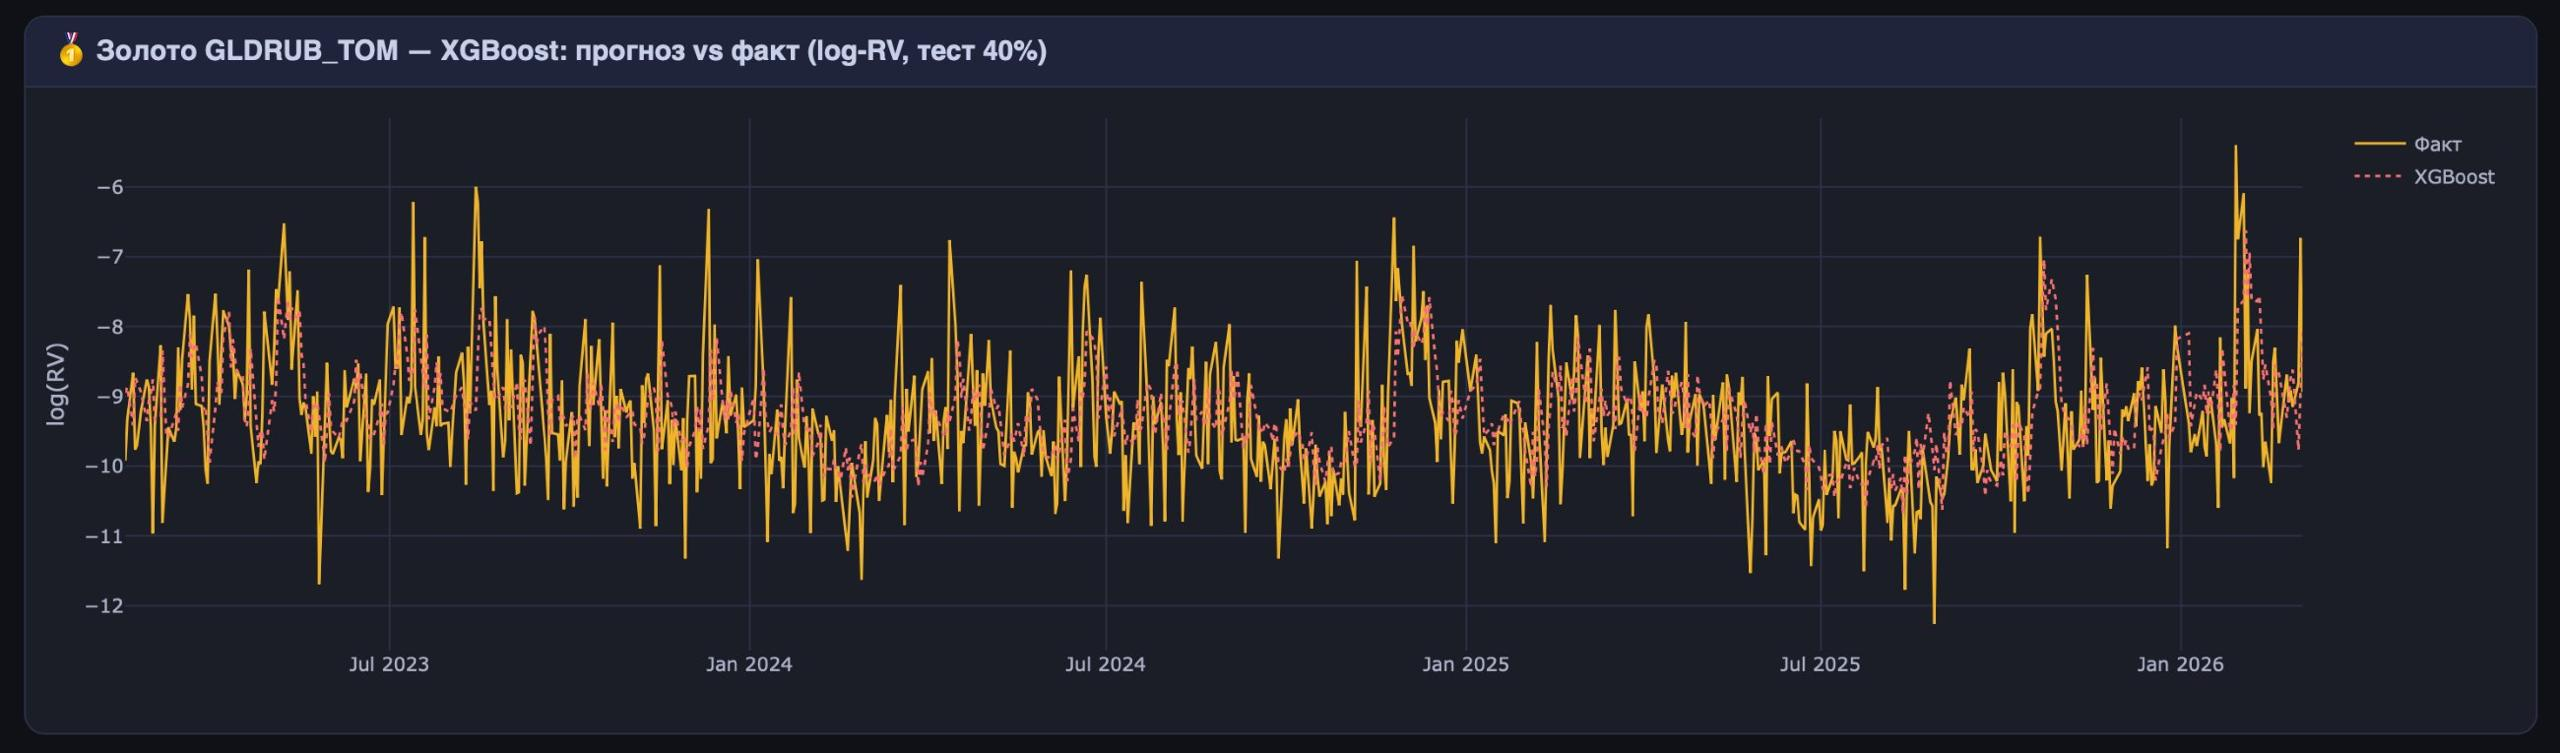
\includegraphics[width=\linewidth]{figures/ui_forecast_gld.png}\\[4pt]
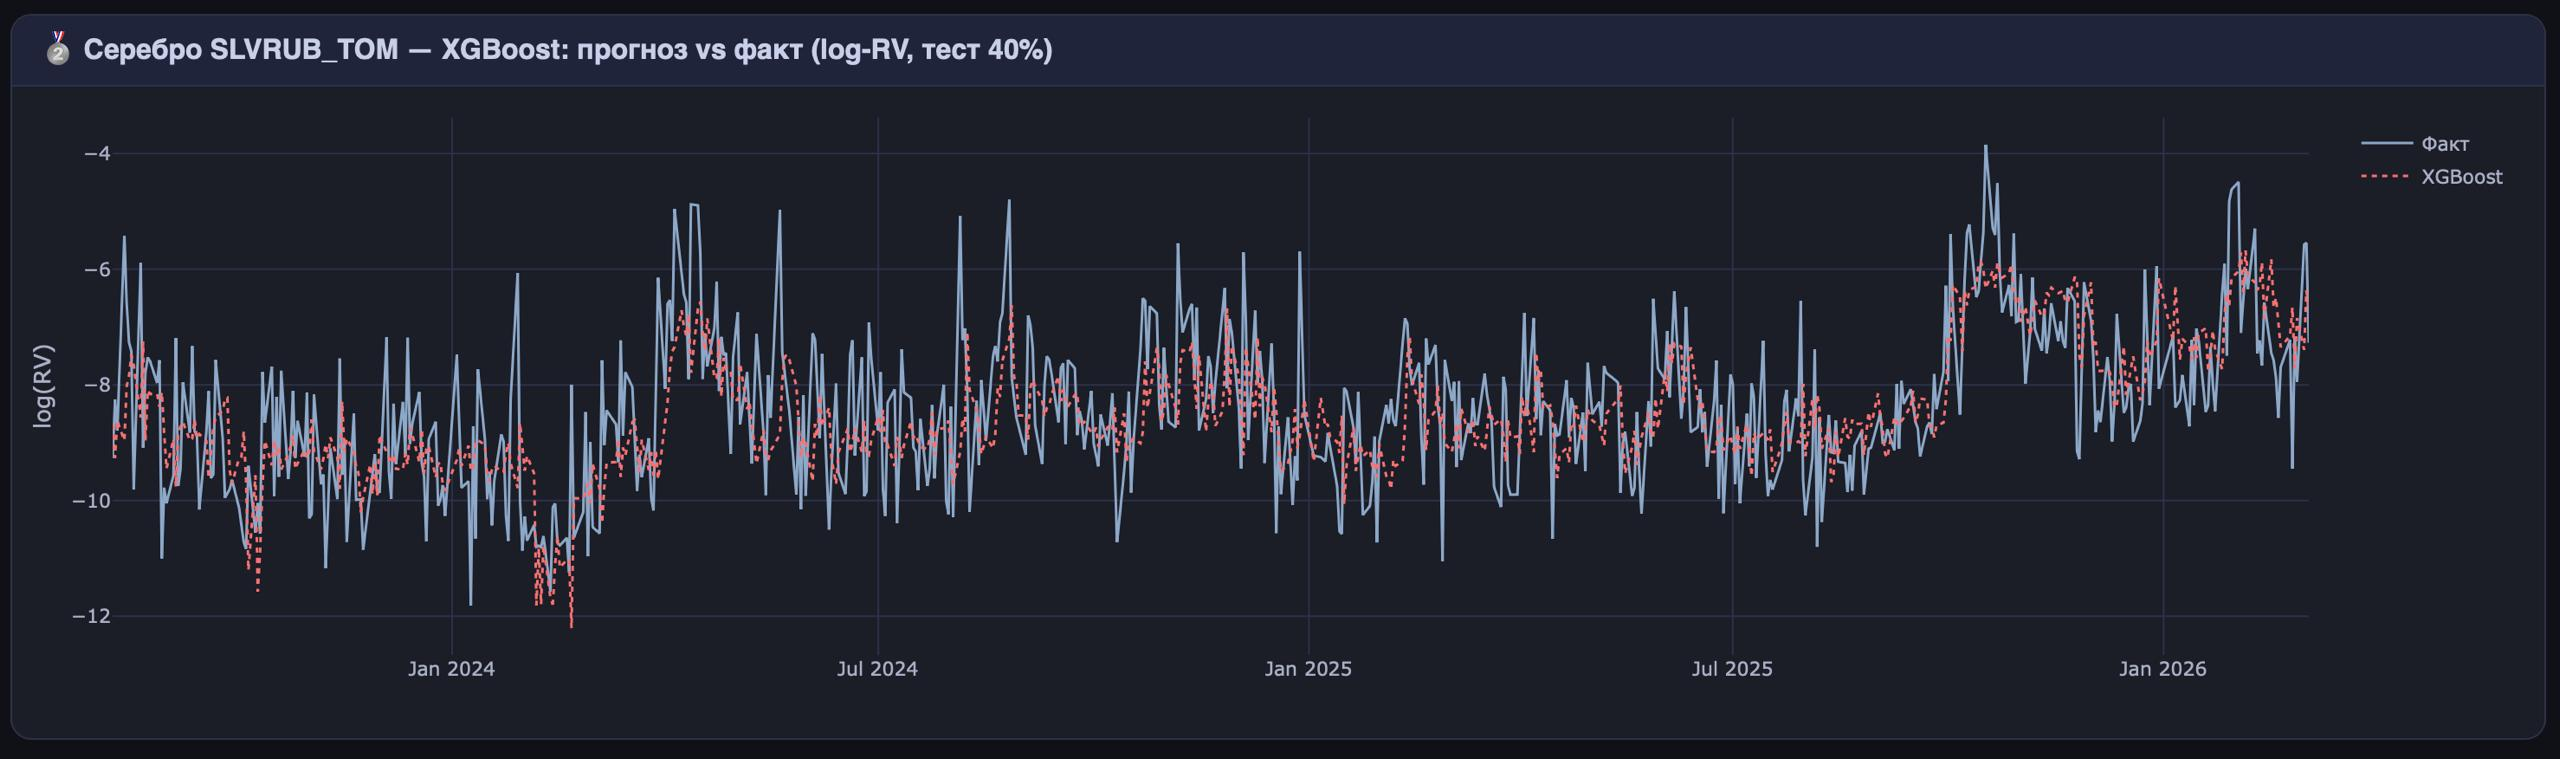
\includegraphics[width=\linewidth]{figures/ui_forecast_slv.png}
\caption{Страница прогноза веб-интерфейса: сопоставление фактической
реализованной волатильности (log-RV) с прогнозом XGBoost на тестовой
выборке для золота (GLDRUB\_TOM, сверху) и серебра (SLVRUB\_TOM, снизу).}
\label{fig:ui_forecast}
\end{figure}
